\chapter{Caso de Estudio} \label{chap:CasoDeEstudio}
En este capítulo vamos a analizar una serie de operaciones que desarrollamos con el fin de mostrar varios de los aspectos claves que brinda la herramienta. Para ello, planteamos el estudio de diversos tipos y fuentes de datos de aplicaciones de Mensajería y Redes Sociales dado que estas dos categorías representan hoy en día una proporción muy importante de la actividad promedio de los usuarios de dispositivos móviles.

Para la categoría de Mensajería, estudiaremos los tipos de datos Email y SMS utilizando como fuentes de datos las aplicaciones de Email y SMS que brinda Android por defecto.

Para la categoría de Redes Sociales, estudiaremos el tipo de dato \emph{Contact} utilizando como fuentes de datos las aplicaciones de Facebook, WhatsApp y la agenda de contactos de Android.

De esta forma, en la primera mitad del capítulo veremos diversos aspectos importantes que se deben tener en cuenta al implementar operaciones y varias formas en que la herramienta facilita el desarrollo de las mismas. Luego, en la segunda mitad describiremos los conjuntos de datos utilizados para probar las operaciones y veremos un ejemplo de ejecución de las mismas.

\section{Mensajería}
Consideremos las operaciones antes descritas para datos de tipo SMS e Email. En el caso de ambas, hay un par de observaciones importantes a hacer:
\begin{itemize}
\item CybOX provee objetos predefinidos que permiten representar a sus tipos de datos (\emph{SMSMessage} e \emph{EmailMessage} respectivamente).
\item Podemos utilizar el \emph{ApplicationExtractor} que es provisto por la herramienta por defecto (como se menciona en el \autoref{app:GuiaExtension}) dado que nuestro interés se encuentra en datos de aplicación.
\end{itemize}

De esta forma, si tomamos en cuenta los pasos que se enumeran en el \autoref{app:GuiaExtension}, los únicos componentes que debemos implementar para dichas operaciones son sus respectivos inspectors.

El inspector de SMS representa un caso sencillo, por lo cual nos servirá para describir los aspectos básicos que debemos tener en cuenta al desarrollar un inspector. Mientras que en el caso del inspector de Email veremos algunos aspectos más avanzados que agrega.

\subsection{Inspector de SMS} \label{InspectorSMS}
Este inspector extrae el tipo de dato \emph{SMSMessage} definido en CybOX. La fuente de datos considerada es la aplicación por defecto de SMS de Android. A continuación veamos cuales son los puntos que tuvimos en cuenta para su implementación.

Para obtener la información sobre los SMS, debemos acceder a una base de datos SQLite (en este caso la misma se llama \emph{mmssms.db}). Para esto, podemos hacer uso del módulo \texttt{sqlite3} disponible en las bibliotecas estándar de Python.

Los campos del objeto \emph{SMSMessage} que utilizamos para representar los datos disponibles en la aplicación de SMS de Android fueron los siguientes:
\clearpage

\footnotesize
    \renewcommand*{\arraystretch}{1.4}
    \begin{longtable}{ | >{\bfseries}m{5cm} | >{\itshape}m{5.0cm} | >{\itshape}c |}
    \hline
    \BlackCell{Nombre} & \BlackCell{Descripción} \\ \hline \hline
    Sender\_Phone\_Number & Número del emisor. \\ \hline
    Recipient\_Phone\_Number & Número del receptor. \\ \hline
    Sent\_DateTime & Número del destinatario. \\ \hline
    Body & Fecha de envío. \\ \hline
    Length & Cantidad de caracteres del mensaje. \\ \hline
    \caption {Campos utilizados del objeto SMSMessage}
    \end{longtable}
    \normalsize

Con respecto a los números del emisor y receptor del SMS, estos no son almacenados explícitamente como tales por parte de la aplicación. La misma almacena el número del dispositivo con el que interactúa. Esto es, en caso de un SMS saliente se guarda el número de quién lo recibe y en caso de un SMS entrante se guarda el número del emisor. La aplicación no almacena el número del dispositivo en la cual opera.

Por otro lado, recordemos que todo inspector debe retornar un conjunto de objetos (que llamamos source objects) que representen los archivos de los cuales se obtuvo la información de los objetos examinados. Para simplificar esta tarea desarrollamos un método llamado \texttt{create\_file\_object} en una clase auxiliar. El mismo puede ser utilizado por cualquier inspector pasándole una ruta a un archivo y obteniendo como resultado un objeto CybOX File que contiene la información sobre el mismo.

En este caso, el inspector de SMS utilizará como archivo de fuente de datos únicamente al archivo de base de datos (\emph{mmssms.db}). Veamos la representación XML del objeto File que obtenemos como resultado de utilizar el método auxiliar antes mencionado:
\newline

\begin{xml} 
<cybox:Observable id="example:Observable-26">
    <cybox:Object id="example:File-3">
        <cybox:Properties xsi:type="FileObj:FileObjectType">
            <FileObj:File_Name>mmssms.db</FileObj:File_Name>
            <FileObj:File_Path>
/data/data/com.android.providers.telephony/databases/mmssms.db
            </FileObj:File_Path>
            <FileObj:File_Extension>.db</FileObj:File_Extension>
            <FileObj:Size_In_Bytes>102400</FileObj:Size_In_Bytes>
            <FileObj:File_Format>
                SQLite 3.x database, user version 57
            </FileObj:File_Format>
            <FileObj:Hashes>
                <cyboxCommon:Hash>
                    <cyboxCommon:Type xsi:type="cyboxVocabs:HashNameVocab-1.0">
                        SHA256
                    </cyboxCommon:Type>
                    <cyboxCommon:Simple_Hash_Value>
a75af1ff214920c74aea4958e683c17558baa7464be316e5ecc82eb9296ae707
                    </cyboxCommon:Simple_Hash_Value>
                </cyboxCommon:Hash>
            </FileObj:Hashes>
        </cybox:Properties>
    </cybox:Object>
</cybox:Observable>
\end{xml}

Finalmente, deseamos indicar los archivos de donde fue extraída la información presente en cada uno de los objetos examinados. De este modo, a cada objeto \emph{SMSMessage} creado se le agrega en sus RelatedObjects las referencias a los objetos de los cuales se obtuvo la información. Esto el inspector lo puede realizar utilizando el método \texttt{add\_related} del objeto CybOX de la siguiente forma:
\newline

\begin{python}
sms.add_related(source_objects[0],
                ObjectRelationship.TERM_EXTRACTED_FROM,
                inline=False)
\end{python}

La representación en XML de uno de los objetos \emph{SMSMessage} producidos se ve de la siguiente forma:
\newline

\begin{xml} 
<cybox:Observable id="example:Observable-18">
    <cybox:Object id="example:SMSMessage-1">
        <cybox:Properties xsi:type="SMSMessageObj:SMSMessageObjectType">
            <SMSMessageObj:Sender_Phone_Number>
                099555236
            </SMSMessageObj:Sender_Phone_Number>
            <SMSMessageObj:Sent_DateTime>
                2015-02-21T17:39:28
            </SMSMessageObj:Sent_DateTime>
            <SMSMessageObj:Body>Hola, todo bien?</SMSMessageObj:Body>
            <SMSMessageObj:Length>16</SMSMessageObj:Length>
        </cybox:Properties>
        <cybox:Related_Objects>
            <cybox:Related_Object idref="example:File-3">
                <cybox:Relationship xsi:type="cyboxVocabs:ObjectRelationshipVocab-1.1">
                    Extracted_From
                </cybox:Relationship>
            </cybox:Related_Object>
        </cybox:Related_Objects>
    </cybox:Object>
</cybox:Observable>
\end{xml}

\subsection{Inspector de Email}
Este inspector extrae el tipo de dato \emph{EmailMessage} definido en CybOX. La fuente de datos considerada es la aplicación por defecto de Email de Android. Los campos del objeto \emph{EmailMessage} que utiliza el inspector para representar los datos disponibles en la aplicación son los siguientes:
\newline

\footnotesize
    \renewcommand*{\arraystretch}{1.4}
    \begin{longtable}{ | >{\bfseries}m{4cm} | >{\itshape}m{6.0cm} | >{\itshape}c |}
    \hline
    \BlackCell{Nombre} & \BlackCell{Descripción} \\ \hline \hline
    Header & Cabezales del email. \\ \hline
    Raw Body & Cuerpo completo en crudo. \\ \hline
    Attachments & Referencias a los archivos adjuntos del email. \\ \hline
    \caption {Campos utilizados del objeto EmailMessage}
    \label{objetoEmailMessage}
    \end{longtable}
    \normalsize
    
A diferencia del caso anterior, ahora existen dos bases de datos, \emph{EmailProvider.db} e \emph{EmailProviderBody.db}, a las cuales debemos acceder para obtener información sobre los correos. En la primera se encuentran almacenados los cabezales de los mismos, mientras que en la segunda se encuentran almacenados sus cuerpos. A su vez, los correos también pueden tener archivos adjuntos asociados los cuales se encuentran almacenados en otros directorios (según se describe en \cite{attchprov}). 

Para cada objeto \emph{EmailMessage} que representa un correo, el inspector debe agregar los objetos que representan archivos adjuntos de dicho email al campo \emph{attachements} (Ver cuadro \ref{objetoEmailMessage}). Estos objetos también deben ser agregados al conjunto de source objects que devuelve el inspector.

Al conjunto de source objects que devuelve el inspector debemos agregar tanto los objetos que representan las dos bases de datos utilizadas como todos los objetos que representan los archivos adjuntos de los emails representados.

De esta forma, un objeto \emph{EmailMessage} podrá contar con más de un objeto relacionado. El primero será el objeto que referencia al archivo de la base de datos, \emph{EmailProvider.db}, que contiene los cabezales de los correos. En caso que de que email contenga un cuerpo, el segundo objeto relacionado es el archivo que representa la base de datos \emph{EmailProviderBody.db}, la cual contiene los cuerpos de los correos.

A continuación se muestra la representación en XML de uno de los objetos \emph{EmailMessage}:
\newline

\begin{xml}
<cybox:Observable id="example:Observable-110">
  <cybox:Object id="example:EmailMessage-8">
    <cybox:Properties xsi:type="EmailMessageObj:EmailMessageObjectType">
      <EmailMessageObj:Header>
        <EmailMessageObj:To>
          <EmailMessageObj:Recipient
    xsi:type="AddressObj:AddressObjectType"category="e-mail">
            <AddressObj:Address_Value>
                to@gmail.com
            </AddressObj:Address_Value>
          </EmailMessageObj:Recipient>
        </EmailMessageObj:To>
        <EmailMessageObj:From xsi:type="AddressObj:AddressObjectType" category="e-mail">
          <AddressObj:Address_Value>
            Google &lt;no-reply@accounts.google.com&gt;
          </AddressObj:Address_Value>
        </EmailMessageObj:From>
        <EmailMessageObj:Subject>
            New sign-in from Firefox on Windows
        </EmailMessageObj:Subject>
        <EmailMessageObj:Date>
            2015-06-10T20:16:25
        </EmailMessageObj:Date>
        <EmailMessageObj:Message_ID>
    &lt;Y6KoAJHcll5r46_XiM1UcQ@notifications.google.com&gt;
        </EmailMessageObj:Message_ID>
        <EmailMessageObj:Content_Type>
          text/html
        </EmailMessageObj:Content_Type>
      </EmailMessageObj:Header>
      <EmailMessageObj:Raw_Body>
        -- El cuerpo del mensaje fue removido para 
        -- mejorar la lectura de la estructura.
      </EmailMessageObj:Raw_Body>
      <EmailMessageObj:Attachments>
        <EmailMessageObj:File object_reference="example:File-85"/>
        <EmailMessageObj:File object_reference="example:File-87"/>
        <EmailMessageObj:File object_reference="example:File-89"/>
        <EmailMessageObj:File object_reference="example:File-91"/>
        <EmailMessageObj:File object_reference="example:File-93"/>
      </EmailMessageObj:Attachments>
    </cybox:Properties>
    <cybox:Related_Objects>
      <cybox:Related_Object idref="example:File-3">
        <cybox:Relationship xsi:type="cyboxVocabs:ObjectRelationshipVocab-1.1">
          Extracted_From
        </cybox:Relationship>
      </cybox:Related_Object>
      <cybox:Related_Object idref="example:File-73">
        <cybox:Relationship xsi:type="cyboxVocabs:ObjectRelationshipVocab-1.1">
          Extracted_From
        </cybox:Relationship>
      </cybox:Related_Object>
    </cybox:Related_Objects>
  </cybox:Object>
</cybox:Observable>
\end{xml}

De forma recíproca, a los objetos que representan archivos adjuntos le agregamos como objeto relacionado al objeto \emph{EmailMessage} dentro del cual venía el mismo. Esto el inspector lo realiza de la siguiente forma:
\newline

\begin{python}
att.add_related(email,
             ObjectRelationship.TERM_CONTAINED_WITHIN, 
             inline=False)
\end{python}

Veamos un ejemplo de un objeto CybOX que representa un archivo adjunto en su representación XML:
\newline

\begin{xml}
<cybox:Observable id="example:Observable-144">
  <cybox:Object id="example:File-85">
    <cybox:Properties xsi:type="FileObj:FileObjectType">
      <FileObj:File_Name>2</FileObj:File_Name>
      <FileObj:File_Path>
/data/data/com.android.email/databases/1.db_att/2
      </FileObj:File_Path>
      <FileObj:File_Extension/>
      <FileObj:Size_In_Bytes>
        1692
      </FileObj:Size_In_Bytes>
      <FileObj:File_Format>
        PNG image data, 144 x 144, 
        8-bit/color RGBA, non-interlaced
      </FileObj:File_Format>
      <FileObj:Hashes>
        <cyboxCommon:Hash>
          <cyboxCommon:Type xsi:type="cyboxVocabs:HashNameVocab-1.0">
            SHA256
          </cyboxCommon:Type>
          <cyboxCommon:Simple_Hash_Value>
c6d6285d9fdc4074c366ef0544f1b6b23d7604183f74c8b9cc6d0cc56b1db4c0
          </cyboxCommon:Simple_Hash_Value>
        </cyboxCommon:Hash>
      </FileObj:Hashes>
    </cybox:Properties>
    <cybox:Related_Objects>
      <cybox:Related_Object idref="example:EmailMessage-8">
        <cybox:Relationship xsi:type="cyboxVocabs:ObjectRelationshipVocab-1.1">
          Contained_Within
        </cybox:Relationship>
      </cybox:Related_Object>
    </cybox:Related_Objects>
  </cybox:Object>
</cybox:Observable>
\end{xml}

\section{Redes sociales} \label{RedesSociales}
Las aplicaciones de redes sociales suelen manejar un gran volumen de datos personales, lo cual las hace una fuente de datos muy interesante. Desafortunadamente, CybOX no cuenta con objetos predefinidos que puedan representar adecuadamente a muchos de los tipos de datos que solemos encontrar en las mismas. Frente a esta situación, recordemos que contamos con la alternativa de extender las capacidades de CybOX diseñando un nuevo objeto CybOX para representar un nuevo tipo de dato.

De esta forma, analizamos varias aplicaciones de redes sociales con el objetivo de encontrar un tipo de datos lo suficientemente interesante que fuera utilizado por las mismas. Observamos que uno de los conceptos en común que manejan es el de contacto. Si bien el nombre utilizado para el mismo varía dependiendo del contexto de cada una (amigo, vínculo, seguidor, etc), éste forma parte imprescindible en todas ellas. Por lo tanto, decidimos diseñar un nuevo objeto CybOX llamado \emph{Contact} para representarlo.

Los datos asociados a un contacto en cada red social particular varían pero un cierto conjunto de datos básicos es compartido a través de todas ellas (incluso en aplicaciones fuera de esta categoría como es la agenda del teléfono).

En la siguiente tabla podemos observar los campos del objeto \emph{Contact}:
\newline

\footnotesize
    \renewcommand*{\arraystretch}{1.4}
    \begin{longtable}{ | >{\bfseries}m{3cm} | >{\itshape}m{7.0cm} | >{\itshape}c |}
    \hline
    \BlackCell{Nombre} & \BlackCell{Descripción} \\ \hline \hline
    Display name & Nombre completo del contacto. \\ \hline
    First name & Nombre del contacto. \\ \hline
    Last name & Apellido del contacto. \\ \hline
    Phone number & Teléfono del contacto. \\ \hline
    Email & Email del contacto. \\ \hline
    Profile picture & URI a la imagen de perfil. \\ \hline
    Birthday & Fecha del cumpleaños con formato yyyy-mm-dd. \\ \hline
    \caption {Campos del objeto Contact}
    \end{longtable}
    \normalsize
    
La forma en que debemos implementar un nuevo objeto CybOX se puede ver en detalle en la sección \ref{nuevoTipoDeDatos} del \autoref{app:GuiaExtension}.

A continuación veremos cómo el tipo de dato \emph{Contact} se ajusta a diferentes aplicaciones. También veremos qué otros detalles, además de contar con un nuevo objeto CybOX, debimos tener en cuenta al implementar cada uno de los inspectors.

\subsection{Inspector de Facebook}
Debido a que la aplicación de Facebook ha variado mucho en los últimos años, nos encontramos con la necesidad de desarrollar un mecanismo para obtener la versión de la aplicación a partir de los datos extraídos de la misma.

Al utilizar el \emph{ApplicationExtractor}, además de obtener el directorio de datos privados de la aplicación, también obtenemos el APK de la aplicación indicada. De esta forma, si examinamos el \emph{AndroidManifest} contenido en el APK, podremos obtener la versión de la aplicación dado que esta información se encuentra declarada en el mismo mediante la propiedad \emph{android:versionName} \cite{amvername}.

Para realizar esto hay un detalle que debemos resolver primero, y es el hecho de que el archivo \emph{AndroidManifest} contenido en el APK se encuentra en formato binario. Para obtener datos del mismo, podemos utilizar la misma herramienta que es utilizada por la toolchain de Android para convertirlo de su formato original en XML a binario. Esto se realiza de la siguiente forma:
\newline

\begin{bash}
aapt dump badging Facebook.apk
package: name='com.facebook.katana' versionCode='11209847' versionName='35.0.0.48.273' platformBuildVersionName='5.0-1521886'
\end{bash}

Vemos que entre los datos devueltos por la herramienta, se encuentra el número de versión.

De esta forma, podemos invocar dicha herramienta desde el inspector para obtener la versión de la aplicación a partir del APK que se encuentra en los datos extraídos, y decidir qué acciones tomar en base a este dato. Con el fin de facilitar el desarrollo mediante la reutilización de código de uso frecuente, este mecanismo decidimos incluirlo en el módulo \emph{inspectors\_helper} mediante el método \texttt{get\_app\_version\_name}.

Veamos ahora algunos detalles de la estructura que presenta la aplicación de Facebook.

Al igual que las aplicaciones de SMS e Email ya vistas, la aplicación Facebook cuenta una base de datos (de nombre \emph{fb.db}) en la cual se encuentra toda la información que precisamos relevante a contactos (o como Facebook los llama en este caso, amigos).

En el caso de Facebook, contamos con información de todos los campos representados en el objeto \emph{Contact} y la misma se encuentra almacenada en una única tabla (friends). Por lo tanto, la obtención de los datos de contactos de Facebook resulta muy directa.

Veamos para la representación en XML para un objeto \emph{Contact} de Facebook:
\newline

\begin{xml}
<cybox:Observable id="example:Observable-26">
  <cybox:Object id="example:Contact-1">
    <cybox:Properties xsi:type="CustomObj:CustomObjectType" 
      custom_name="Contact">
      <cyboxCommon:Custom_Properties>
        <cyboxCommon:Property name="display_name">
          Joe Bautista
        </cyboxCommon:Property>
        <cyboxCommon:Property name="first_name">
          Joe
        </cyboxCommon:Property>
        <cyboxCommon:Property name="last_name">
          Bautista
        </cyboxCommon:Property>
        <cyboxCommon:Property name="phone_number">
          +639157175318
        </cyboxCommon:Property>
        <cyboxCommon:Property name="email">
          jobau518@yahoo.com
        </cyboxCommon:Property>
        <cyboxCommon:Property name="profile_picture">
          http://profile.ak.fbcdn.net/hprofile-ak-ash2/
            49302_1337617745_5617_q.jpg
        </cyboxCommon:Property>
        <cyboxCommon:Property name="birthday">
          1947-5-18
        </cyboxCommon:Property>
      </cyboxCommon:Custom_Properties>
    </cybox:Properties>
    <cybox:Related_Objects>
      <cybox:Related_Object idref="example:File-3">
        <cybox:Relationship 
          xsi:type="cyboxVocabs:ObjectRelationshipVocab-1.1">
          Extracted_From
        </cybox:Relationship>
      </cybox:Related_Object>
    </cybox:Related_Objects>
  </cybox:Object>
</cybox:Observable>
\end{xml}

\subsection{Inspectors de WhatsApp}
La primera diferencia que podemos percibir con Facebook, es que WhatsApp no almacena información acerca de los emails ni fecha de cumpleaños de los contactos.

En segunda instancia, hay una pequeña diferencia en cuanto a la imagen de perfil. A diferencia de Facebook en el cual la base de datos contiene una referencia a una URL, WhatsApp almacena un identificador que hace referencia a un archivo local. Para esto, en el campo \emph{profile\_picture} utilizamos la ruta al archivo en el dispositivo prefijando el scheme \emph{file://}.

\subsection{Inspector de la agenda telefónica de Android}
En el caso de la agenda telefónica, el único dato que no almacena la aplicación es la fecha de cumpleaños del contacto.

La única dificultad que presenta la implementación del inspector de este caso es el hecho de que cuenta con un esquema de base de datos bastante más complejo que los anteriores. Para poder obtener la información de un contacto, es necesario acceder a múltiples tablas \emph{contacts}, \emph{people}, \emph{contact\_methods} y \emph{phones}.

\section{Un extractor alternativo}
\subsection{Motivación}
El hecho de que las operaciones cuentan por separado con los mecanismo de extracción e inspección, otorga a la herramienta la flexibilidad en cómo implementar las operaciones. De esta forma, en el caso de la extracción de datos de aplicaciones podemos llegar a implementar un extractor alternativo al extractor, mencionado en el \autoref{app:GuiaExtension}, que la herramienta brinda por defecto. Esto permite que si lo deseamos podamos cambiar operaciones que utilizan el extractor de datos de aplicaciones por defecto que brindamos, por este nuevo extractor.

¿Para qué implementar un extractor de datos de aplicaciones alternativo si los datos que obtiene son los mismos? La diferencia está en que el método que utilicemos para realizar la extracción nos puede brindar otros beneficios. En este caso, el \emph{ApplicationExtractor} que brinda la herramienta por defecto tiene la particularidad que precisa acceso root al dispositivo.

Como vimos en la subsección \ref{alternativasRooting} del capítulo Estado del Arte, el mecanismo del comando \texttt{adb backup} proporciona una excelente alternativa para obtener los datos privados de las aplicaciones sin necesidad de contar con root en el dispositivo. El único inconveniente que presenta este mecanismo es que las aplicaciones pueden decidir si desean permitir o no el backup de sus datos y deshabilitar de esta forma este mecanismo. De todas formas, en nuestra experiencia la mayoría de las aplicaciones esta funcionalidad se encuentra habilitada dado que éste es su valor por defecto.

\subsection{Detalles de implementación}
Al ejecutar el comando \texttt{adb backup}, el usuario debe interactuar con el dispositivo y aceptar que se realice el backup de los datos. Este comando empaqueta y comprime los datos encontrados dentro del directorio de la aplicación (junto con su APK si así se lo indicamos). El nombre de los directorios de bases de datos, shared preferences y archivos es cambiado por el comando de backup (Por ejemplo, el directorio \emph{shared\_prefs} pasa a llamarse \emph{sp}).

En \cite{unpkbckp} se describe en detalle el formato utilizado para crear los archivos de backup de Android.

La implementación de este nuevo extractor, al cual llamamos \emph{AdbBackupExtractor}, consta de tres etapas:

\begin{enumerate}
\item Mediante el comando \texttt{adb backup} se obtiene el archivo \emph{backup.ab}.
\item A este archivo, primero le quitamos el cabezal (que corresponde a los primeros 24 bytes). Luego, descomprimimos su contenido utilizando la biblioteca estándar \emph{zlib} de Python, obteniendo un archivo tar. Finalmente, desempaquetamos el contenido del archivo tar utilizando la biblioteca estándar \emph{tarfile} de Python.
\item De forma de preservar los nombres de directorios que son utilizados por las aplicaciones debemos renombrarlos a sus nombre originales, como ya vimos.
\end{enumerate}

\section{Datos de prueba}
Con el fin de obtener resultados significativos en las pruebas de las operaciones implementadas, buscamos utilizar datos de entrada que fueran representativos de un uso real de los dispositivos móviles. Para esto, utilizamos dos \emph{disk images} de muestra que brinda Oxygen Forensics (en su sitio web \cite{oxigforn}) con el objetivo de simular casos reales para evaluar el funcionamiento de su suite de software forense.

Las especificaciones de los dispositivos correspondientes a las imágenes obtenidas son las siguientes:
\newline

\footnotesize
    \renewcommand*{\arraystretch}{1.4}
    \begin{longtable}{|>{\centering\arraybackslash}p{3.5cm}|>{\centering\arraybackslash}p{3cm}|>{\centering\arraybackslash}p{3cm}|}
    \hline
    \BlackCell{} & \BlackCell{Número de modelo} & \BlackCell{Versión de Android} \\ \hline \hline
    Samsung Galaxy Mini & GT-S5570 & 2.2 \\ \hline
    HTC EVO 3D & X515m & 2.3 \\ \hline
    \caption {Dispositivos de prueba utilizados}
    \end{longtable}
    \normalsize
    
Las particiones obtenidas de cada dispositivo fueron \emph{userdata} y \emph{sdcard}.

Como observamos, ambas imágenes datan de ya hace un par de años si juzgamos por la versión de Android que disponían los dispositivos. Lo mismo sucede con las versiones de las aplicaciones móviles utilizadas. Es importante además tener en cuenta que únicamente contamos con los datos de las aplicaciones y no con los del sistema.

Dado que los extractors utilizados en el caso de estudio realizar la extracción de los datos directamente del dispositivo, debemos tener una forma de implantar los datos obtenidos en un dispositivo para luego realizar las pruebas con la herramienta.

La opción ideal sería poder recrear los sistemas originales de los dispositivos de los cuales obtuvimos los datos en una máquina virtual de forma que las aplicaciones funcionen tal cual lo hacían en sus dispositivos original. Esta resulta ser una tarea muy difícil, en particular por los hechos antes mencionados de que no contamos con los datos del sistema y tampoco con los APKs de las aplicaciones.

Optamos por utilizar un emulador con una imagen estándar de Android en la cual implantamos los datos en sus correspondientes directorios del filesystem. En particular, el emulador utilizado fue Genymotion \cite{genymotion} con la imagen de la versión de Android 4.3 provista por ellos. Cabe destacar que la imagen provista ya se encontraba con acceso root, por lo cual no debimos realizar ningún otro paso antes de implantar los datos.

Con el fin de automatizar este proceso, creamos un script Python que se encarga de implantar un \emph{dataset}. Específicamente, le llamamos \emph{dataset} a un archivo \emph{tar} que contiene tanto APKs de aplicaciones como directorios correspondientes a los que se encuentran en la ruta \emph{/data/data} de un dispositivo. De esta forma, al especificar el nombre de uno de estos archivos el script toma los directorios contenidos en el archivo tar y los copia a la ruta \emph{/data/data} del dispositivo e instala los apks de aplicaciones. Para ello simplemente utiliza los comandos \texttt{adb install} y \texttt{adb push}.

Los \emph{datasets} con los que contamos corresponden a los antes descritos sólo que únicamente contienen los datos de las aplicaciones utilizadas en el caso de estudio, estas son Facebook, WhatsApp y las aplicaciones por defecto de email, SMS y contactos de Android. Además en el caso de las aplicaciones de terceros (Facebook y WhatsApp) contienen los APKs de sus últimas versiones.

\section{Ejecución de la herramieta}
Para terminar, veremos un ejemplo de ejecución interactiva de la herramienta en la cual primero utilizaremos el script visto en la sección anterior para cargar los datos en un emulador y luego realizaremos varias extracciones de datos utilizando varias de las operaciones que se desarrollaron a lo largo de este capítulo.

Comenzamos ejecutando el script \texttt{load\_data\_sets} utilizando el \emph{dataset} correspondiente al dispositivo HTC Evo 3D adquirido.
\newline

\begin{bash}
$ ./load_data_sets.py --ds HTC_Evo_3D
Installing 'com.facebook.katana-1.apk' into the device...
Installing 'com.whatsapp-1.apk' into the device...
Pushing 'com.whatsapp' data into the device...
Pushing 'com.android.providers.telephony' data into the device...
Pushing 'com.facebook.katana' data into the device...
Pushing 'com.android.providers.contacts' data into the device...
The data set was pushed successfully.
\end{bash}

Una vez que contamos con los datos cargados en el emulador, iniciamos la herramienta en modo interactivo de la siguiente forma:
\newline

\begin{bash}
$ ./andi.py 
Android Inspector v1.0
\end{bash}

El primer comando que vamos a utilizar es \texttt{set\_device\_info} para indicarle a \emph{Android Inspector} el modelo del dispositivo emulado que se encuentra conectado y la versión de Android que está corriendo.
\newline

\begin{bash}
(Andi) set_device_info -m GT-I9300 -v 4.3
Device model 'GT-I9300' running Android version '4.3' was set as the current device information.
\end{bash}

De esta forma, cuando utilicemos los comandos \texttt{list} y \texttt{execute}, la información del dispositivo recién establecida será tomada en cuenta de forma implícita tanto para filtrar por las operaciones soportadas en el caso del primero como para pasarle esta información a cada operación que ejecuta en el caso del segundo (recordemos que la misma es utilizada por los inspectors al ejecutar una operación).

Veamos la información de las operaciones que se encuentran disponibles para el dispositivo que establecimos utilizando el comando \texttt{list}.
\newline

\begin{bash}
(Andi) list
Name                   Data type     
---------------------  ------------  
EmailMessageAOSPEmail  EmailMessage  
SmsMessageAOSPSms      SMSMessage    
ContactFacebook        Contact       
ContactWhatsApp        Contact       
ContactAOSPAgenda      Contact       

Data Source                                                
---------------------------------------------------------  
Application{package_name:com.android.email}                
Application{package_name:com.android.providers.telephony}  
Application{package_name:com.facebook.katana}              
Application{package_name:com.whatsapp}                     
Application{package_name:com.android.providers.contacts}   

Supported devices           Supported Ver.
----------------------------------------  
[GT-I9300, XT1053]          [2.3.7-5.1.1]
[GT-I9300, XT1053]          [2.2.0-4.4.4]
[GT-I9300, Nexus5, XT1053]  [4.1-4.4.4]
[GT-I9300, XT1053]          [4.1-4.4.4]
[GT-I9300, XT1053]          [2.3-4.4.4]
\end{bash}

Ahora que conocemos las operaciones que podemos ejecutar para este dispositivo podemos empezar a extraer los datos que deseamos. Por ejemplo, para extraer los mensajes de texto de la aplicación por defecto de mensajería de Android observamos que tenemos la operación \emph{EmailMessageAOSPEmail} que desarrollamos en la sección \ref{InspectorSMS}. De esa forma, podemos ejecutarla pasándole el nombre de la misma al comando \texttt{execute}.
\newline

\begin{bash}
(Andi) execute -op SmsMessageAOSPSms 

[1/1] Executing 'SmsMessageAOSPSms': 
Fetching '/system/app/TelephonyProvider.apk' file...
Fetching '/data/data/com.android.providers.telephony' directory...
COMPLETED. Data stored to 'results/SmsMessageAOSPSms_20150826_081415'.

1 operation(s) completed successfully.
\end{bash}

La salida del comando en este caso nos muestra que la operación que ejecutamos completó exitosamente. Además, nos indica el directorio en dónde quedaron almacenados tanto los datos extraídos como los archivos XML de CybOX conteniendo los datos examinados.

El comando \texttt{execute} permite ejecutar múltiples operaciones, una detrás de la otra, si especificamos varias. Por ejemplo, podemos ejecutar las operaciones \emph{ContactFacebook} y \emph{ContactWhatsApp} que desarrollamos en la sección \ref{RedesSociales} para extraer los datos de contactos de estas dos aplicaciones.
\newline

\begin{bash}
(Andi) execute -op ContactFacebook ContactWhatsApp

[1/2] Executing 'ContactFacebook': 
Fetching '/data/app/com.facebook.katana-1.apk' file...
Fetching '/data/data/com.facebook.katana' directory...
COMPLETED. Data stored to 'results/ContactFacebook_20150826_084055'.

[2/2] Executing 'ContactWhatsApp': 
Fetching '/data/app/com.whatsapp-1.apk' file...
Fetching '/data/data/com.whatsapp' directory...
COMPLETED. Data stored to 'results/ContactWhatsApp_20150826_084107'.

2 operation(s) completed successfully.
\end{bash}

Utilizando el comando \texttt{tree} de Unix podemos observar la estructura de los directorios con los datos resultantes de las tres operaciones que ejecutamos.
\newline

\begin{bash}
$ tree -L 3
.
|__ ContactFacebook_20150826_084055
|   |__ extracted_data
|   |   |__ com.facebook.katana-1.apk
|   |   |__ databases
|   |__ inspected_data.xml
|   |__ source_data.xml
|__ ContactWhatsApp_20150826_084107
|   |__ extracted_data
|   |   |__ com.whatsapp-1.apk
|   |   |__ databases
|   |   |__ files
|   |   |__ shared_prefs
|   |__ inspected_data.xml
|   |__ source_data.xml
|__ SmsMessageAOSPSms_20150826_081415
    |__ extracted_data
    |   |__ app_parts
    |   |__ databases
    |   |__ shared_prefs
    |   |__ TelephonyProvider.apk
    |__ inspected_data.xml
    |__ source_data.xml
\end{bash}

Sería interesante observar una porción de los archivos XML que contienen los objetos CybOX producidos por las operaciones. Para esto, podemos utilizar la herramienta \texttt{cybox-to-html} \cite{stix-to-html} que produce una representación de los XML más clara en HTML. A continuación veremos un par de extractos de los objetos CybOX que contienen los archivos \emph{source\_data.xml} y \emph{inspected\_data.xml} correspondientes a la ejecución de la operación \emph{ContactFacebook}.

En el archivo \emph{source\_data.xml} podemos encontrar el siguiente objeto File:
\newline

\begin{figure}[H]
    \begin{center}
        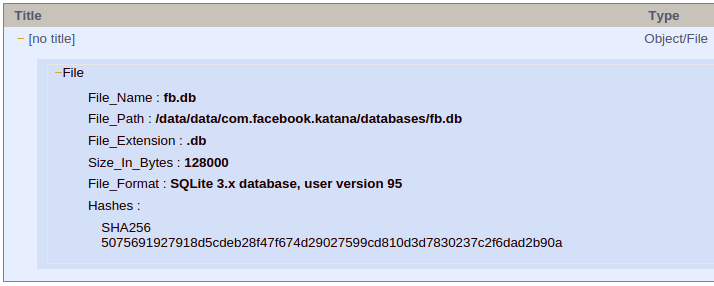
\includegraphics[width=\textwidth]{figures/FbDBFileObject}
        \caption{Objeto \emph{File} que representa al archivo de base de datos \emph{fb.db} del cual se extrajeron los datos sobre los contactos de Facebook.}
    \end{center}
\end{figure}

En tanto, en el archivo \emph{inspected\_data.xml} podemos encontrar una serie de objetos \emph{Contact} representando a cada uno de los contactos de Facebook obtenidos. Veamos un par de ellos:
\newline

\begin{figure}[H]
    \begin{center}
        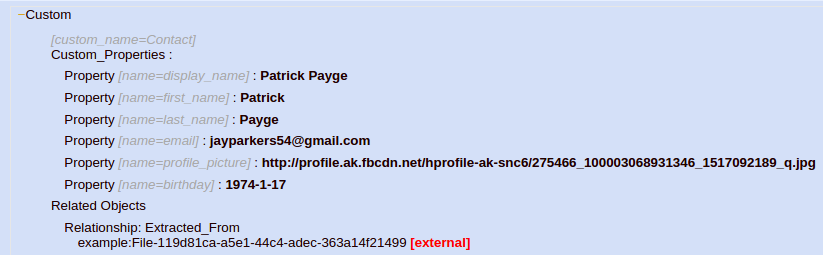
\includegraphics[width=\textwidth]{figures/contact1}
        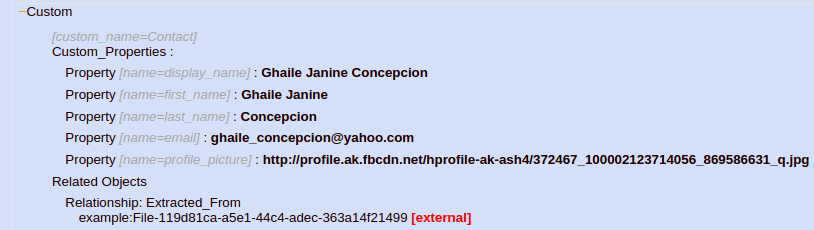
\includegraphics[width=\textwidth]{figures/contact2}
        \caption{Información de los dos primeros objetos \emph{Contact} del archivo \emph{inspected\_data.xml}.}
    \end{center}
\end{figure}

De esta forma, vimos una sesión completa de ejecución de la herramienta en la cual realizamos diversas extracciones de datos y examinamos su representación. Queda en manos del investigador forense cómo utilizar esta información expresada mediante el lenguaje CybOX para realizar diversos análisis a partir de la misma.